\documentclass[12pt,preprint]{aastex}
\newcommand{\ch}[1]{\textbf{\color{red}#1}}

\begin{document}
\tolerance=10000
\def\simlt{\lower.5ex\hbox{$\; \buildrel < \over \sim \;$}}
\def\simgt{\lower.5ex\hbox{$\; \buildrel > \over \sim \;$}}

\title {ASTRONOMY WITH THE 21-CM LINE; \\ SOME MICROWAVE ELECTRONICS \\ \today}

\tableofcontents

\section{GOALS} \begin{itemize}

\item Understand time: UT/UTC, PST, LST, Julian day. 

\item Measure a 21-cm line power spectrum from atomic Hydrogen in the
  Milky Way.

\item Combine data by averaging, medianing.

\item Remove the instrumental contribution to the spectrum.

\item Use rotation matrices to convert among various spherical
  coordinate systems.

\item Produce spectra with velocities expressed in various coordinate
  systems.

\item Representing spectra by Gaussian components.

\item Learn the basics of transmission lines and waveguides.

\item Learn about reflections and minimizing them with impedance
  matching.

\item Derive propagation velocities by measuring the wavelength of
  standing waves.

\item Empirically explore waveguides and their cutoff properties.

\item Use linear and nonlinear least-squares fitting to squeeze the best
  results from your data.

\end{itemize}

\section{SCHEDULE}
\begin{enumerate}
\item {\it The First Week. For class JD=2458163:} % XXX change this each year
Finish \S\ref{radioastro} and \S \ref{analysis}, and understand \S
  \ref{jultime}. Be prepared for `show and tell'.

\item {\it The Second Week. For class JD=2458170:} % XXX change this each year
Finish \S \ref{meas2}, \S \ref{expt}, and \S \ref{secondweek}. 

\item {\it The Third Week. For class JD=2458177:} Write up your formal
  report. And finish what you couldn't get done during the first two
  weeks!
\end{enumerate}

\section{YOUR LAB REPORT}

The lab reports, as always, are written by {\it individuals}. 

The microwave and other electronics is such an important part of this
lab that you should include a block diagram of the telescope electronics
in your lab report. You can prepare this either by either hand or
computer. If by hand, you'll have to scan your drawing to get a file you can
insert into your report's tex file. If by computer, you can use your
favorite software for making line drawings.  Although it is dated, {\tt xfig}
comes installed on Linux, so that's another option.  In \LaTeX, the line
{\tt \textbackslash usepackage\{graphicx\}} will give you the {\tt \textbackslash includegraphics} command,
which you can use to put images of various file types into your document.  Common
formats are {\tt png} (good for lines), {\tt jpg} (good for images), and {\tt pdf}
(best for plots/line figures).  Each of these formats has a different way of representing
graphics.  In particular, {\tt pdf} (and {\tt ps}) can represent plots and figures 
in {\it vector graphic} form --- as instructions for drawing each line of the figure.  This 
form, which contrasts {\it bitmap} image formats like {\tt png} and {\tt jpg}, is
infinitely scalable and never has pixelization issues, making it ideal for representing
figures in a paper.

The real work in this lab is the analysis, so it provides the ideal
opportunity for you to flex your programming muscles. Accordingly, {\it
  each individual} needs to write her/his own software. And this
software needs to be documented, preferably using Python docstrings
(see, for example, the documentation in the code of {\tt ugradio.pico}, which
shows up if you type, e.g., {\tt ugradio.pico.capture\_data?} at the Python prompt.)
{\it Include this
  documentation} (but not the rest of the software) {\it as part of your lab
report}. Also include a brief description of how to run your software;
tell me the subdirectory where your software can be found; and make sure
I can look at those subdirectories by setting the permissions so that
they are readable by `world'. 

\section{WHAT TIME IS IT?} \label{jultime}

\subsection{Whaddya Mean by Time?}

Coordinated Universal Time (UTC) is the Civil Time\footnote{You use
  Civil Time when you set your alarm clock for getting up in the
  morning.} in Greenwich, England, which is 8 hours ahead of (larger
than) PST. Remember that in the middle of this course, we switch from
PST to PDT; PST=UTC - 8 hr, while PDT=UTC - 7 hr). Think of Civil time
as Solar time, because the 24-hour period is the same as that of the
Sun.

Think of Sidereal Time as ``star time''; it tells when a
particular star (not the Sun) is visible. The 24-hour sidereal time period is a
bit shorter than the 24-hour Solar time period---$1 \over 356$ less, to
be almost exact. This is a little less than 4 minutes per day.  Local Sidereal Time
depends on your location on Earth (in particular, your longitude), and tells you
what right ascension (the ``longitude" coordinate for stars) is directly overhead
at a particular moment.

The Julian Day is a sequential numbering of Solar days. As such, it
uniquely specifies the date without the need for any complications such
as months (with their nonsensical definitions\footnote{``Thirty days
  hath September\dots''}), leap years, etc. It begins at noon (UT=12hr)
in Greenwich, so it is 12 hours out of phase with UT. But the
international date line is 12 hours away from UT, so the JD is in sync
with humankind's definition of `when the day begins'. JD=0 begins at
Greenwich noon on 1 Jan --4713.  The Julian day is a double-precision
float: it contains the time as the fractional part of the day. It's not
just an integer day number. The current JD is about 
2458163. % XXX change this each year

The Modified Julian Day is a shorter version of Julian Day. MJD is 12
hours out of sync with JD, so it is in sync with local time at
Greenwich. MJD=0 occurs at 0 hr UT on 17 Nov 1858.  The current MJD is
about 58162. % XXX change this each year

\subsection{ Software---Some Useful Python Procedures for Time Conversion}

Python has several built-in modules for dealing with time, including {\tt time}, {\tt datetime}.
Astronomers, however, have historically been the best time-keepers on the planet.  For
astronomy-quality time routines, {\tt astropy.time}, part of the {\tt astropy} package, is
the industry standard.
These routines are based on GSFC {\tt ct2lst.pro}. LST tells when a star
is overhead, so its rate of passage depends on the Earth's spin. The
Earth is constantly slowing owing to tidal friction produced by the
Moon. The conversion between Civil Time and LST has to be adjusted
periodically by inserting `leap seconds', so unless you keep up with
this, the conversion will be off by a few seconds. 

You need to know your
longitude to calculate LST. NCH has \\
{\tt (lat,lon) = (37.8732, -122.2573)},  Note that {\tt lon = -122.2573 = (360 - 122.2573) = 237.7427}. 
For all procedures mentioned here, these are the defaults.

\begin{verbatim}
local_now = ugradio.timing.local_time() # current local time as a string

ut_now = ugradio.timing.utc() # current UTC as a string

ut_now = ugradio.timing.unix_time() # seconds since 1 January 1970

julian_now = ugradio.timing.julian_date() # current julian day (which \
        contains the current time, too--it's not just an integer \
        number. 
                                                                               
lst_now = ugradio.timing.lst() # current LST at NCH
                                                                               
lst_julian = ugradio.timing.lst(jd) # LST for the specified Julian day                                                             
                                                                               
ut_julian = ugradio.timing.unix_time(jd) # seconds since 1/1/1970 for given JD
                                                                               
julian_ut = ugradio.timing.julian_date(ut) # julian day for given unix time
\end{verbatim}

\section{HANDOUTS} \label{handouts}
\begin{enumerate}
\item A second-level IDL tutorial. {\tt idldatatypes.pdf} ``QUICK IDL % XXX update for python
  TUTORIAL NUMBER TWO: IDL DATATYPES AND ORGANIZATIONAL STRUCTURES'' For
  this lab you use complex numbers, matrices and matrix
  math, and structures. This handout describes the complete set and, in
  addition, how numbers are stored and represented, and how accurate
  they are. {\it You need to know all of this stuff!}

\item The complete story of producing calibrated spectral line shapes
  and intensities:``CALIBRATING THE INTENSITY AND SHAPE OF SPECTRAL
  LINES''. This handout is {\it optional} because the steps discussed in
  this lab writeup (what you're reading now) are sufficient, but
  if they are unclear or you want to know more, this writeup has it all.

\item What physical quantity are we measuring? Sure, it's power received
  by the telescope. But what does that mean about the source being
  observed? It's all about specific intensity, usually denoted $I$:
  ``SPECIFIC INTENSITY: THE FOUNT OF ALL KNOWLEDGE! or $I,
    \ T_B, \ T_{SYS}, \ T_{RCVR}, \ S,$ and $\tau \Delta \nu$. You need
  to understand these topics to interpret your measurements.

\item Astronomical coordinate transformations with Rotation Matrices:
  {\tt ay120coord.pdf} ``AY121 CHEAT-SHEET FOR SPHERICAL COORDINATE % XXX check pdf name
  TRANSFORMATION''. converting among Az/El, Ha/Dec, Ra/Dec, L/B. {\it
    You need to know all of this stuff!}

\item You can do this lab without doing any textbook-type reading\dots
  but then you wouldn't gain the insight from the highly readable and
  well-written text by Ramo, Whinnery, and van Duzer (RWvD), {\it Fields
    and Waves in Communication Electronics}. This is a great book
  because it contains commentary on applications to modern devices
  (e.g., the discussions of transmission lines carrying pulses from one
  piece of computer hardware to another are very nice).  Reading this
  book is {\it optional}, but in any case see notes below in \S
  \ref{RWvD}.

\end{enumerate}

\section{IN THE LAB: YOUR FIRST 21-cm LINE MEASUREMENT (First Week; by GROUPS)} 
\label{radioastro}

This week we will use the techniques we explored in Lab 1 to measure the
21-cm line (colloquially known among astronomers as the {\it
  HI}---that's {\it H - ``Roman numeral I'', pronounced ``H-one''}) line
shape, velocity, and intensity using the big horn on Campbell's roof.
Most of the measured power comes from our own electronics, not the HI
line.  It's often called ``noise'', and we need to get rid of this
instrumental contribution. We also need to obtain the correct line shape
and intensity.

We'll measure the 21-cm line twice. For the first, the goal is to master
the technical aspects and familiarize ourselves with the system and
procedures, so instead of worrying about where to point the horn we'll
just take whatever position happens to be overhead. For the second (\S
\ref{meas2}), we'll manually point the horn to a designated position and
make a calibrated profile to compare with a well-established standard
profile measurement.

\subsection{The Receiving System}
We will use a double-heterodyne system for the 21-cm line at 1420.4 MHz.
`Double heterodyne' means we have two mixing stages.  It works
like this: \begin{enumerate}

\item For the first mixer, we use the ordinary DSB technique. Suppose we
  use an l.o.\ (the `first local oscillator') at 1230.0 MHz so that the
  difference frequency is 190.4 MHz and the sum frequency is 2650.4 MHz.
  We use a 20 MHz-wide bandpass filter centered at 190 MHz to obliterate
  the sum frequency, so we are left with a replica of the 21-cm line
  that is centered at 190.4 MHz instead of 1420.4 MHz.

\item For the second mixer, we use the SSB technique. The second
  l.o.\ has frequency 190.0 MHz, so the output frequencies are positive
  and negative, centered about zero; this is called `baseband'. In the
  absence of Doppler shift, we are left with the line centered at 0.4
  MHz. However, the line is shifted and broadened by Galactic rotation
  and the Earth's orbital velocity, so it covers a range of frequency
  of, for example, $1420.2 \pm 0.5$ MHz. We use a low-pass filter with a
  cutoff frequency of, say, 2 MHz to
  eliminate aliasing, sample the complex signal, and Fourier transform
  to calculate the power spectrum. We take many power spectra and
  average them to reduce the noise.

\end{enumerate}

\subsection{Your Measurement}

Before taking actual data, it's important to do some basic system
checks: (1) make sure the signal levels are OK and (2) experimentally
determine which way frequency increases on your power spectra.
\begin{enumerate}

\item Set the system up as you will be using it to observe. Point the
  horn to zenith to reduce interference and thermal noise.  Take some
data.  How fast must you sample? 

\item Look at the range of sample values by plotting a bunch of
  them. Best is to make a histogram, which you can do using Python's {\tt
    numpy.histogram} function.  
      To get its documentation,
    type {\tt numpy.histogram?}.
    The sampled numbers should cover plenty of bits;
  quantization should be only barely, or not at all, visibly evident in
  the histogram. Adjust {\tt volt\_range} in the call to {\tt pico.capture\_data}
  accordingly.

The
  histogram shape should look like a well-known function. Which
  function? Does it?

\item Insert a test signal so that it appears in the upper sideband and
take some data; then change the test signal frequency so it's in the
lower sideband.  You'll use this to make sure that the SSB mixer is
doing its job properly, and to determine whether the frequency axis
is flipped or not.

\item The horn is a gigantic rain bucket. You won't see any
  astronomical signal unless you dump it!

\end{enumerate}

Having determined that the system basics work, it's time to do
astronomy! For this first measurement the main goal is to master the
technical aspects, so use whatever position happens to be overhead and
point the horn straight up. The line will be strongest---strong enough
to see visually---for the approximate range LST = 19 - 6 hr.

It is most convenient to use temperature units---Kelvins---for the power
that we measure. Accordingly, the power that we measure is called the
`System Temperature' $T_{sys}$. It's a function of frequency and has two
kinds of behavior: the `continuum', which is devoid of spectral features
and changes very slowly with frequency; and the `line', which in this
case is the 21-cm line and it changes relatively rapidly with frequency---hence our
desire to obtain the line shape.

The System Temperature has two contributions: (1) the dominant contribution
  from our electronics, which we call the `Receiver Temperature' $T_R$;
  and (2) the contribution from sky, being picked up by the antenna, the
  `Antenna Temperature' $T_A$. Thus $T_{sys}=T_R + T_A$, and usually
  $T_R \gg T_A$. 

Our horn is equipped with an old, noisy first amplifier so $T_R \sim
300$ K; in contrast, our Leuschner telescope is much better, with $T_R
\sim 50$ K. The antenna temperature comes from the Cosmic Background,
with brightness temperature ($T_{B,CMB} = 2.7$ K); from
interstellar/intergalactic space with brightness temperature
$T_{B,astron}$ (usually no more than a few K in the continuum and up to
about 100 K in the HI line); and the Earth's atmosphere with brightness
temperature $T_{B,atm}$, perhaps a few K at the HI line frequency. So
off the HI line we have $T_A \sim 10$ K and on the HI line, in the
Galactic plane where it is strongest, we have $T_A \sim 100$ K.

We'll take two sets of data: (1) a long integration to measure the line
{\it shape}. and (2) a short integration so we can calibrate the line's
{\it intensity.}


\begin{enumerate}

\item 
The measured power spectrum {\it shape} is dominated by the
frequency-limiting filters acting on the System Temperature. To see the
line, which is weak, we need to correct for these filter shapes, which
we do by obtaining a spectrum containing no line. Accordingly, to get
the shape we take two spectra: one with the line present (the `online'
spectrum $s_{online}$) and one with the line not present (the `offline'
spectrum $s_{offline}$).

We could obtain the online
  spectrum by centering the line and making a measurement; then changing
  the first l.o.\ frequency so that the line shifts either completely
  outside the band (this is called `frequency switching'), or partway
  over but is still in the band (called 'in-band frequency
  switching'). The latter is better because you are always looking at
  the line; you end up with more measurements of it and thus get better sig/noise.

To accomplish this, take a spectrum with the line roughly in the upper
half of the baseband spectrum, and another with it centered roughly in
the lower half. Use the first as the `online' and the second as the
`offline' spectrum for the upper half. Similarly, for the lower half,
use the second as the `online' and the first for the `offline'.  (The HI
line frequency is 1420.4058 MHz).

You can change the l.o.\ frequency in software: use {\tt set\_hp}. % XXX track down this function

The line is weak, and you'll need to take lots of spectra. Recall that
{\tt pico.capture\_data} obtains a specified number of blocks ({\tt nblocks}),
each of which has 16000 datapoints and writes them all out into a single
file. Suppose you decide to obtain 10000 spectra. You might be tempted
to do it in one fell swoop by setting {\tt nblocks=10000}. That
will work, but be aware that it will take about 5 minutes or more. You
might want to instead take ten sets with {\tt nblocks=1000} so you can do a
sanity check on your data without waiting for what seems like forever. 

\item Intensity calibration requires a second pair of measurements,
  which can be short. Easiest is probably to take one with the horn
  looking at a known blackbody and one looking at cold sky. What's a
  convenient blackbody? You! And your friends! So take one short
  measurement with the horn pointing straight up at cold sky and the
  other with as many people as you can find standing in front of it and
  `filling the aperture'. (Or you can use rainwater). Call these spectra
  $s_{coldsky}$ and $s_{300K}$.

\end{enumerate}

\section{THE ANALYSIS (First Week; by INDIVIDUALS)} \label{analysis}

\subsection{Take a Suitable Average/Median}
Consider, first, the $s_{online}$ and $s_{offline}$ spectra, from which
you can find the line shape. There are many individual spectra, 10000 in
our above example. You need to combine these to make a single spectrum
for each measurement. You can do this by averaging the power spectra
(use {\tt numpy}'s {\tt mean} function) or by taking the medians (use {\tt numpy}'s
{\tt median} function). The former gives a less noisy result, but the
latter handles time-variable interference better; use both and compare
the results. Even after combining the 10000 spectra, the resulting
spectrum will still look noisy.  You can reduce the noise by averaging
over channels---by `smoothing' the spectrum. This reduces the noise, but
degrades the spectral resolution, so you have to make a compromise on
how many channels to smooth over. To decide, realize that the HI line is
never narrower than about 1 km/s, so it's OK to degrade the frequency
resolution to, say, 1 or 2 kHz. Again, you do the smoothing by averaging
(by using {\tt numpy.mean} ) or medianing (by using {\tt
  numpy.median}), and again try both to see what happens.

In the smoothed $s_{online}$ spectrum you might not be able to see the
HI line, because the instrumental bandpass dominates the spectrum
shape. The instrumental bandpass is determined mainly by the low-pass
filter, which should fall smoothly to zero as the frequency
increases. Does it? If not, should you worry about aliasing?

\subsection{Get the Line Shape}

You can remove the instrumental bandpass, and thus get the shape
of the line (but not the intensity), by taking the ratio 

\begin{equation}
shape = {s_{online} \over s_{offline}} \ .
\end{equation}
%
This is the {\it first} factor (i.e., the shape) in equation
(13) in the spectral-line handout.
%
\subsection{Get the Line Intensity}

To get the line intensity in terms of the calibration noise source,
multiply the shape spectrum by $T_{sys,coldsky}$---the second factor in
the handout's equation (13). We obtain $T_{sys, coldsky}$ by combining
the 300K and caloff spectra as linear proportions, as per equation (15)
in the handout:
%
\begin{equation}
T_{sys, coldsky} = {\sum s_{coldsky} \over \sum(s_{300K} -
  s_{coldsky})} (T_{cal}- T_{sys,coldsky})
\end{equation}
\noindent Here, a sum is over all channels in a spectrum. All this
equation does is to convert measured units, which are digital numbers
from the system, into physically meaningful units, i.e.\ Kelvins. Here,
$T_{cal} = 300$ K, because that's the thermal power you injected by
standing in front of the horn. Since $T_{coldsky} \ll
T_{cal}$, to a first approximation you can neglect it (which is what we
did in the handout). Then the final, intensity-calibrated spectrum is
equation (16) in the handout, namely
\begin{equation}
final \ calibrated \ spectrum = shape \times T_{sys, coldsky}
\end{equation}
%
\subsection{Plotting Intensity vs.\ Frequency---and Velocity} First,
plot your final calibrated spectrum versus the r.f.\ frequency. Next,
plot it versus the Doppler velocity\footnote{Astronomers usually express
  velocities in km s$^{-1}$.}.  Remember that, by astronomical
convention, positive velocity means motion away (remember the expansion
of the Universe!), so

\begin{equation}
{v \over c} = -{\Delta f \over f_0} \ ,
\end{equation}

\noindent where $c$ is the speed of light and $\Delta f$ is the frequency
offset from the line frequency $f_0$\footnote{Radio astronomers, being
  frequency-oriented, use this equation; optical astronomers, of course,
  use something different: ${v \over c} = {\Delta \lambda \over
    \lambda_0}$. At high redshifts the difference becomes significant;
  the optical definition is the usual standard.}. 

\subsection{Finally, Choose a Reference Frame}
You may think we've done it all by this point, but we haven't! We need
to correct the observed velocity for the orbital velocity of the Earth,
and also the Earth's spin. And when observing the Galaxy, it is
customary to express velocities with respect to the `Local Standard of
Rest' (LSR), so that's yet another correction.

Calculate the Doppler correction using {\tt ugdoppler.pro}  % XXX need this
Correct the velocities and plot the spectrum for two
reference frames: (1), the barycentric reference frame, which gives
velocity with respect to the center of mass of the Solar
system\footnote{There's a third system, the Sun system, which gives
  velocity with respect to the center of the Sun. The barycenter lies
  inside the Sun, but not quite at the center, and the barycentric and
  Sun systems are almost the same.}; and (2) the Local Standard of Rest
(LSR), which is approximately the frame that would rotate around the
Galaxy in a circular orbit.

{\it Notes on \verb$ugdoppler$}: \begin{enumerate}

\item You need the celestial coordinates of the source, $(ra, dec)$. How
  to find these for the horn pointing straight up? You could use
  rotation matrices. However, when looking straight up you don't need
  this powerful technique because, quite simply, the Dec is equal to the
  Latitude and RA=LST.

\item You need the Julian day of the observation; see \S \ref{jultime}.

\item You need the observatory coordinates (north latitude and west
  longitude) in degrees; you could enter them with the pair of optional
  input parameters {\tt (nlat, wlong)}, but you don't have to because
  the default values are Campbell Hall's values (which are {\tt nlat=
  37.8732, wlong= 122.2573} degrees).

\end{enumerate}

\section{IN THE LAB: YOUR SECOND 21-cm LINE MEASUREMENT (Second Week; by
  GROUPS)} 
\label{meas2}

Obtain a fully-calibrated spectrum for the horn pointing at Galactic
coordinates $(l,b)=(120^\circ, 0^\circ)$. How do you know where to point
the horn? You definitely do need to use rotation matrices!  See the
handout ``Ay121 Cheat-Sheet for Spherical Coordinate Transformation''
(\S \ref{handouts}). Plot your spectrum versus both the Barycentric and
the LSR velocity. 

\begin{figure}[h!]
\begin{center}
%\vspace{-0.7in}
%       
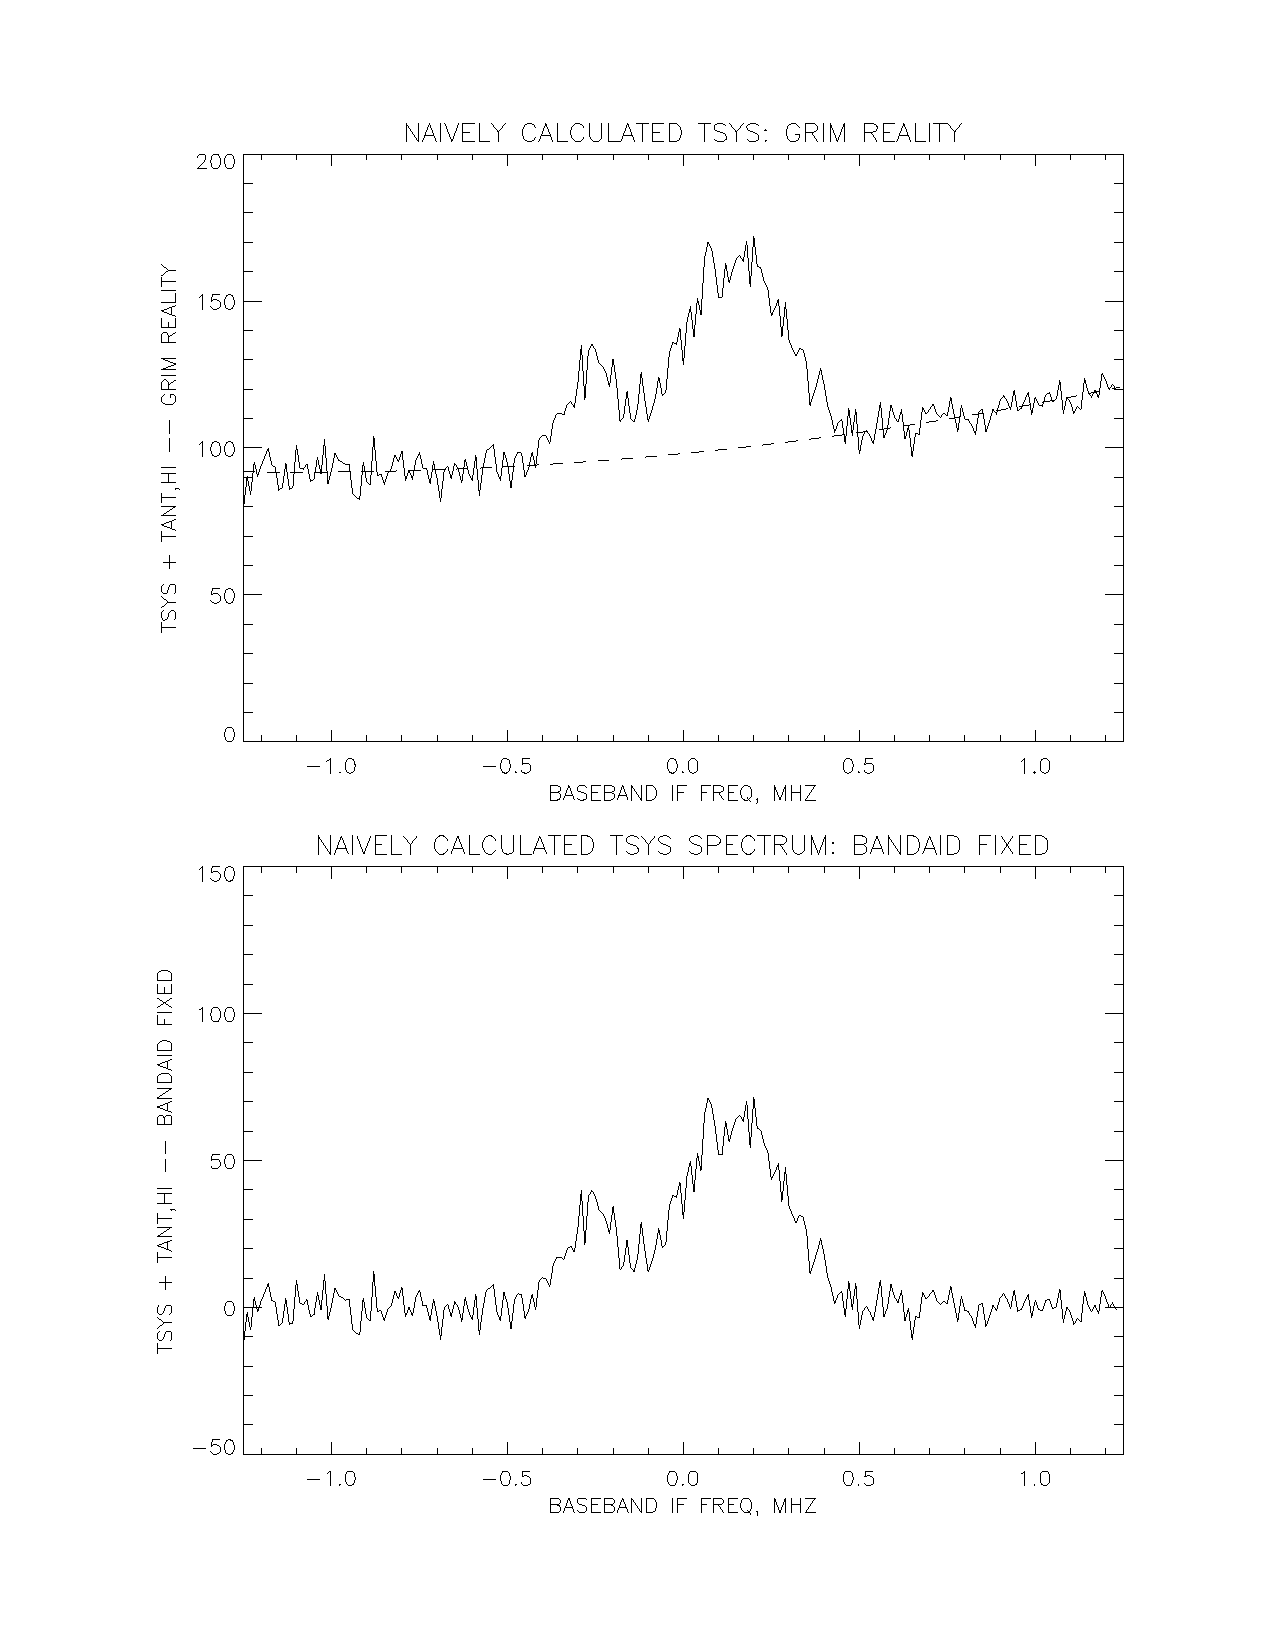
\includegraphics[scale=0.5]{bmp_cal1.pdf}
\end{center}
\vspace{-0.3in}
\caption{\footnotesize A typical raw spectrum with a curvy baseline and
  multiple velocity components. \label{rawspect}}
\end{figure}

Your spectrum will probably look something like that in the top panel of
Figure \ref{rawspect}. There is a zero offset, a curvy `baseline', and
one or more spectral peaks. The curvy baseline comes from nonflat
instrumental response before the first mixer, and can be removed with a
low-order polynomial fit to the off-line channels (the approximate
frequency ranges $-1.2 \rightarrow -0.6$ and $ 0.6 \rightarrow 1.2$
MHz). The dashed line is a second-order polynomial fit to the off-line
channels and the bottom panel has this fit subtracted off.  Here, the
multiple peaks come from HI clouds having different velocities. The
peaks are usually represented as Gaussians with appropriate central
intensities, velocities, and widths.  Fitting Gaussians requires
specifying initial guesses for the component parameters. These guesses
need not be highly accurate. For example, in the bottom panel of Figure
\ref{rawspect}, initial guesses for the two heights, centers, and widths
(FWHM) could be [20, 50], [-0.3, 0.2] MHz, and [0.01, 0.03] MHz.  After
fitting, check to see if the result looks good: if it does not, then
it's usually because you need one or more additional components. It is
common to require a low-level, broad component that produces no obvious
peak; here, the initial guesses might be [20, 50, 10], [-0.3, 0.2, 0.]
MHz, and [0.01, 0.03, 0.07] MHz. 

The procedures you need for these least-squares fits
are: \begin{enumerate}
\item For the polynomial fit, use {\tt numpy.polyfit}

\item For fitting multiple Gaussians, use our home-grown {\tt gaussfit}; for
  evaluating the Gaussians from the parameters produced by {\tt gaussval}, % XXX write this
  use {\tt gaussval}.
\end{enumerate}

In class we'll compare the results from all groups. In this class, we
have never yet---after more than a decade's worth of measurements---had
the results of all groups agree!

\section {IN THE LAB: PROPAGATION VELOCITY MEASUREMENTS WITH SLOTTED LINES AND 
WAVEGUIDES (Second Week; by GROUPS)} \label{expt}

How do you move power or electronic information from one place to
another? Transmission lines (cables) and waveguides are
indispensable. Sounds easy---just connect two things with a wire. But
does this really work? We'll explore cables, waveguides, and reflections
by measuring the Voltage Standing Wave Ratio (VSWR), which results from
interference of incident and reflected waves.

The experimental work and measurements described below should
be done by groups.  The analysis in \S \ref{secondweek} should be done
by individuals. The analysis is nontrivial, so don't delay with the
measurements!

{\boldmath % XXX figure out the procedure for these sections
\subsection {The coax slotted line at C-band ($\sim 3$ GHz)} \label{slotted}
} Set up the slotted coaxial line with the wide-range HP 83712B
synthesizer.  With the far end of the slotted line open, find the
wavelength in the slotted line $\lambda_{sl}$ by measuring the positions
of {\it all} nulls as accurately as you can.  Do the same with the far
end shorted and note the differences.  In particular, note how the
positions of the nulls change when the slotted line is terminated with
an open versus when it is shorted.  Why is this?

From your measurements calculate the velocity [what does ``velocity''
  mean?] in the slotted line by comparing $\lambda_{sl}$ and the
frequency.  First do a quick calculation using your measurements. Then
do it as accurately as possible by using least-squares fitting and
following the advice in \S \ref{slottedls}.  {\it Note:} As it happens,
the velocity is independent of frequency for a coax cable---in contrast
to a waveguide.  If you are so motivated, you can check this
experimentally.

\subsection {The X-band waveguide (7 to 12 GHz)} \label{waveguide}

Now we'll do the same as we did in \S \ref{slotted}, but for X-band
waveguide.  The cutoff frequency for X-band waveguide is about 7
GHz. Pick a suitable frequency and, with the far end of the waveguide
completely open, measure the VSWR; then short the end of the waveguide,
maybe with a piece of aluminum foil or a metal plate, and repeat.  Why
is an open ended waveguide different from an open ended coax cable?

With the end shorted, measure the velocity in the slotted waveguide by
comparing the wavelength and the frequency; do this for several
(half-dozen?) frequencies, including one or two near cutoff, and compare
with theory.  These frequencies should be reasonably closely separated,
say by no more than 1 GHz.  From these measurements, derive the cutoff
wavelength (and thus the waveguide width) as accurately as you can.
Also measure the waveguide dimensions, and compare 
with the width you derived above.

\section {GETTING THE MOST OUT OF YOUR DATA: STATISTICAL ERROR
ANALYSIS (Second Week; by INDIVIDUALS)} \label{secondweek}

\subsection{The coax slotted-line wavelength} \label{lbandcoax} 
\label{slottedls}

	For the measurements of \S \ref{slotted}, you sampled $M$
        cycles of the standing wave in the slotted line. You can
        calculate the wavelength $\lambda_{sl}$ from the distances
        between a single null pair. While this calculation is a good
        estimate, each of your measurements has an error. You have
        measured the distance between $(M-1)$ null pairs. What's the
        best way to combine these measurements so as to obtain the most
        accurate $\lambda_{sl}$?

{\bf (1)} One way is to calculate the wavelength from each neighboring
null {\it pair} and take the average of the $(M-1)$ {\it pair}s.  You
might then apply the usual rule to obtain the uncertainty in the
average, i.e.\ the uncertainty is $(standard \ deviation) \over (M-1)$.
However, this would {\it not be correct}.  Why? (Hint: The answer you
get by averaging the $(M-1)$ pairs is identical to that obtained from a
{\it single} well-chosen non-neighbor pair.  Which one?).  Actually,
this method gives {\it almost} the best estimate of the wavelength.  But
you can do better!

	{\bf (2)} The positions of the nulls should increase linearly
with distance. So if $x_{m}$ is the position of null number $m$, we
should have

\begin{equation}
x_m = A + m {\lambda_{sl} \over 2} \ ,
\end{equation}

\noindent You know $x_m$ and $m$ from measurement and you would like to
derive $A$ and $\lambda_{sl}$. This is a classic least squares problem;
you're fitting a first-degree polynomial, where the unknowns are $A$ and
$\lambda_{sl}$. You can use {\tt numpy.polyfit}.

\subsection{The X-band waveguide}

	RWvD provide a beautiful discussion of the TE$_{10}$ mode in
common rectangular waveguide (in which the ratio of side lengths equals
2).  Most important is their equation 11, which gives the ``guide
wavelength'' $\lambda_g$; we reproduce it here:

\begin{equation} \label{lambdaguide}
\lambda_g = {v_p \over f} = {\lambda_{fs} \over \left[ 1 - (\lambda_{fs}/2a)^2
\right]^{1/2} } \ ,
\end{equation}

\noindent where $\lambda_{fs}$ is the free-space wavelength.  The guide
wavelength is the wavelength within the waveguide, and combining it with
the frequency gives the propagation velocity in the guide. 

Here we want to do a least-squares fit of equation \ref{lambdaguide} to
solve for the waveguide width $a$. Now, you've already measured $a$ with
the caliper. But here the idea is to compare your measurements of the
waveguide cutoff with what theory (that's equation \ref{lambdaguide})
predicts. So you imagine that $a$ is unknown and determine it from your
data on $\lambda_g$ versus the free-space wavelength $\lambda_{fs}$.
Doing this is not as straightforward as above in \S \ref{lbandcoax}
because $\lambda_g$ depends {\it nonlinearly} on $a$. The easiest way to
handle
this problem is by ``brute force'' method, which we will discuss in
class. 

	From your above solution, determine the best-fit value of $a$
and compare it with the value you measured with the caliper.

\section {IN THE MIND: REFERENCE READING} \label{RWvD}

You can do this lab without doing any reading, so this section, which
recommends parts of the highly readable and well-written text by Ramo,
Whinnery, and van Duzer (RWvD), {\it Fields and Waves in Communication
  Electronics}, is optional. If you have the time and inclination to
read, we suggest that you concentrate on the starred items below ({\bf
  ***}).  The notes below refer to the second edition, which should
reside in our lab's bookshelf. The italicized numbers refer to the very
same sections of the book.

\subsection{ Theory of Coaxial Cable}
	
{\bf ***} {\it RWvD \S 5.2:  Introduction: what transmission lines do.}
Basic equations for transmission lines.  Note
equation (14) for the characteristic impedance $Z_0$, which is the ratio
of voltage to current in the line.  This is expressed in ohms, but it is
not ``ordinary resistance'' because voltage and current are out of
phase.  Example 5.2 calculates $Z_0$ for a coax line.  RG58/U, done in
the example, has 50 ohms; so do the cables we use in our system (in
contrast, the TV standard is 75 ohms).  Because of the dielectric in the
cable, the wave (phase) velocity is $\sim 0.7$ that in free space,
making the wavelength in the cable shorter than that in free space; one
needs to account for this when using cables to produce delays in a
signal, as in an interferometer or a quadrature circuit. 

{\bf ***} {\it RWvD \S 5.4: Reflection and transmission at a resistive
discontinuity.} The purpose of a transmission line is to take power from
a source to a load. The load should absorb the power and therefore
should be resistive. If its resistance matches the line impedance, then
all the power transmitted by the line is absorbed by the load. If not,
some is reflected; see their equations (4) and (6). We need to tune our
devices so that they are ``matched'' and reflect no power. 

\subsection{The Theory of Waveguide}
          
{\bf ***} {\it RWvD \S 8.1:  Introduction: general description of
waveguides.} 

{\bf ***} {\it RWvD \S 8.8:  The $TE_{10}$ Mode in a Rectangular
Guide.} A nice, complete discussion of the TE$_{10}$ mode in common
rectangular waveguide (in which the ratio of side lengths equals 2). 
In this mode, E is perpendicular to the long side of the guide
(and also to the longitudinal axis of the guide).  We speak of the
polarization of the waveguide: the guide transmits linear polarization
that is perpendicular to the long side of a waveguide.  When we couple
power into a guide from coax, we do so with a probe that is parallel to
the internal electric field.  When we use a sliding probe to measure
VSWR in a waveguide, the probe extends through a long slot in the broad
side of the waveguide and the probe is parallel to the E field inside
the guide, so it samples the internal E field.  Note {\bf Figure 8.8},
which shows the current flow in the waveguide walls; note that the
current flow down the center of the broad side of the guide is parallel
to the axis of the guide---that is, parallel to the slot that we use for
the probe.  The slot, being parallel to the current flow, does not
interrupt any current flow and has no effect on the internal
distribution of fields in the guide.  Clever!

{\it RWvD \S 8.10.} Makes the analogy between coax cable and waveguide.
A coaxial line can be considered as a waveguide containing walls not
only the outside but also on the inside.  The usual mode that propagates
in coax is the TEM mode.  A TE$_{10}$-like waveguide mode enters for
wavelengths smaller than that given by their equation (4); at this
point, coax lines become basically unusable.  For type N connectors, we
are beginning to approach this limit in our 12 GHz system!

{\it RWvD \S 8.11.} Brief description of how coax lines are coupled to
waveguide. The method depends on which mode you wish to excite. For the
TE$_{10}$ mode, method (b) in Figure 8.11 works well and is almost
universally the one used.

\end{document}

%You can smooth over channels and reduce the noise. For example, suppose you
%want to reduce the the NSAMP channels in the power spectrum $pspect$ to 512
%channels. In IDL there are two
%easy ways to do this: \begin{enumerate}
%
%\item Use IDL's {\tt smooth} function: {\tt newspect = smooth(pspect,
%    NSAMP/512)}. This degrades the resolution, but you will still have
%  NSAMP channels in the output spectrum.
%
%\item Use IDL's {\tt rebin} function: {\tt newspect = rebin(pspect, 512)}.
%  This degrades the resolution and gives you 512 channels channels in the
%  output spectrum.
%\end{enumerate}

